% This is a sample LaTeX input file.  (Version of 12 August 2004.)
%
% A '%' character causes TeX to ignore all remaining text on the line,
% and is used for comments like this one.

\documentclass{article}      % Specifies the document class

\def\Course{Statistical Methods for Machine Learning}
\def\Exam{Assignment 1}
\def\Studentname{
Tudor Dragan (xlq880)\\
Nicolae Mariuta (rqt629)\\
Gabriel Carp
}
\def\Sub_date{\today}
                             % The preamble begins here.
%\title{\bf Principles of Computer Systems Design\\ {\Large Exam}}  % Declares the document's title.
%\author{Tudor Dragan\\}

\title{\textbf{\Course}\\\textbf{\Exam}}
\author{\Studentname}
\date{\Sub_date}      % Deleting this command produces today's date.

\usepackage{verbatimbox}
\usepackage{listings}
\usepackage{color}
\usepackage[]{amsmath}
\usepackage[english]{babel}
\usepackage[utf8]{inputenc}
\usepackage{graphicx}
\usepackage{moreverb}
\usepackage{hyperref}
\usepackage[T1]{fontenc} % font
\usepackage{program}
\usepackage[top=1.5in, bottom=1.5in, left=1.4in, right=1.4in]{geometry}
\usepackage[super]{nth}
\usepackage{fancyhdr}
\usepackage{lastpage}
\usepackage{float}
\usepackage[section]{placeins}
\usepackage[linesnumbered]{algorithm2e}
\usepackage[table,xcdraw]{xcolor}
\definecolor{dkgreen}{rgb}{0,0.6,0}
\definecolor{gray}{rgb}{0.5,0.5,0.5}
\definecolor{mauve}{rgb}{0.58,0,0.82}
\usepackage[table,xcdraw]{xcolor}
\lhead{\textbf{\Course}}
\rhead{\Exam~(Submission: \Sub_date)}

\cfoot{}
\lfoot{\Studentname}
\rfoot{\thepage\ of \pageref{LastPage}}
%\pagestyle{fancy}
\renewcommand{\footrulewidth}{0.4pt}

\lstset{frame=tb,
      language=Java,
      aboveskip=3mm,
      belowskip=3mm,
      showstringspaces=false,
      columns=flexible,
      basicstyle={\small\ttfamily},
      numbers=none,
      numberstyle=\tiny\color{gray},
      keywordstyle=\color{blue},
      commentstyle=\color{dkgreen},
      stringstyle=\color{mauve},
      breakatwhitespace=true
      tabsize=3
}
\newcommand{\ip}[2]{(#1, #2)}
                             % Defines \ip{arg1}{arg2} to mean
                             % (arg1, arg2).

%\newcommand{\ip}[2]{\langle #1 | #2\rangle}
                             % This is an alternative definition of
                             % \ip that is commented out.

\begin{document}             % End of preamble and beginning of text.

\maketitle                   % Produces the title.

\section*{I.2 Probability and Parameter Estimation}
\subsection*{I.2.1 Univariate Gaussian distributions}

\begin{figure}[ht]
\centering
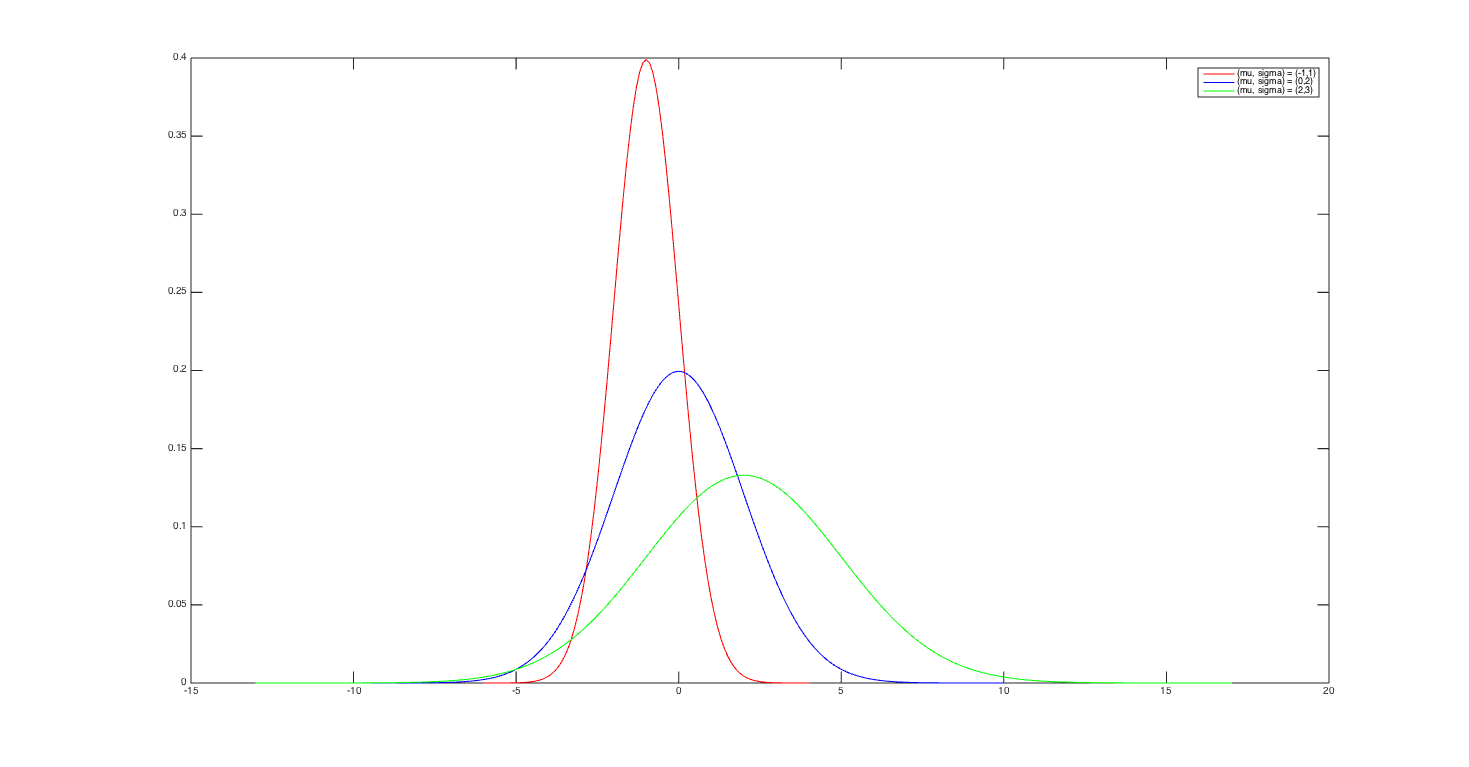
\includegraphics[scale=.3]{img/i21}
\caption{Gaussian distribution for  \label{overflow}}
\[(\mu,\sigma) = (-1, 1), (0, 2), and (2, 3)   \]
\end{figure}

Ox in the gaussian1d function represents the input values and Oy is the output that is calculated by applying the univariate Gaussian Distribution function with means m and standard deviation d.\\

\subsection*{I.2.2 Sampling from a multivariate Gaussian distribution}

\begin{figure}[ht]
\centering
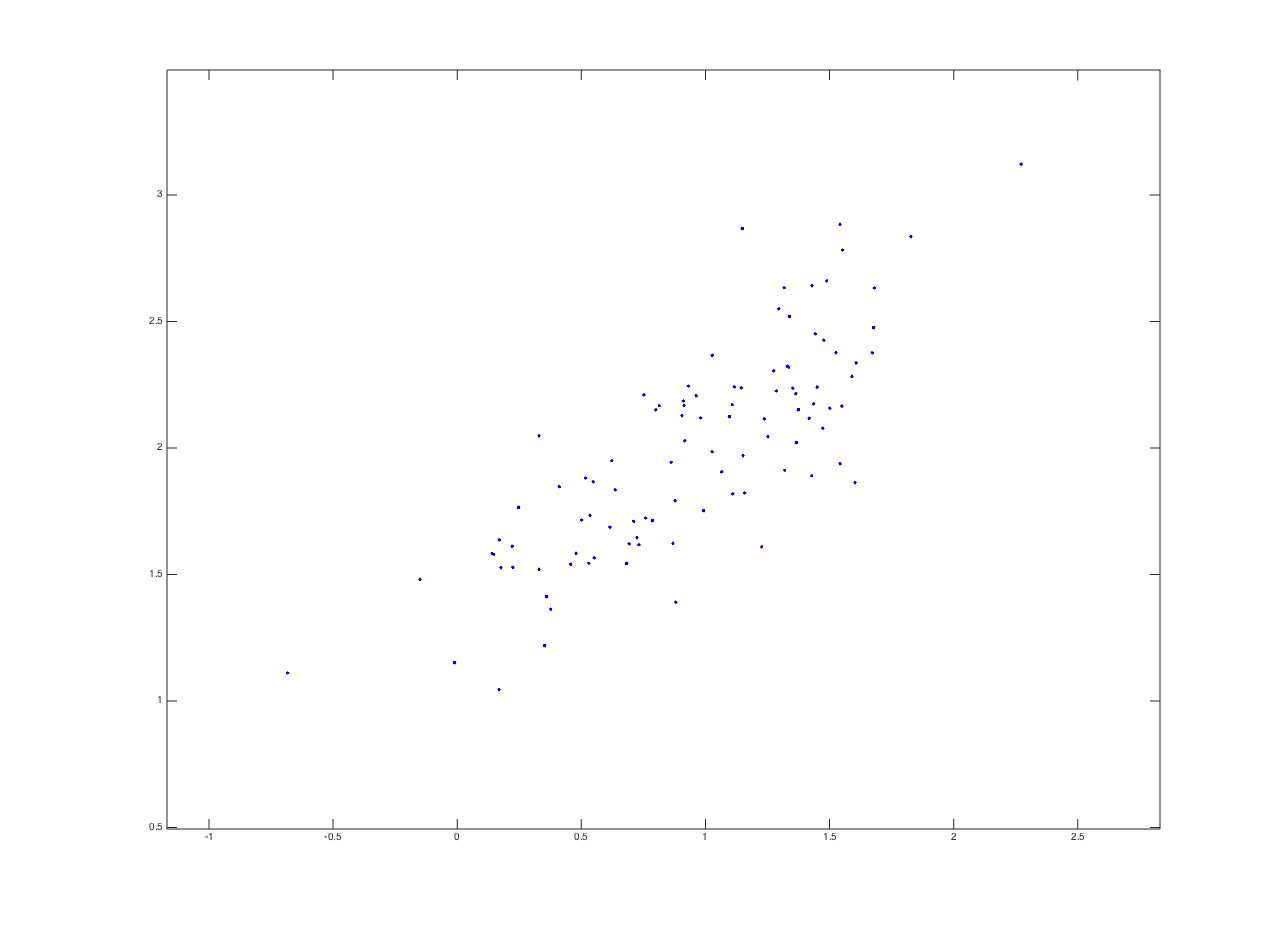
\includegraphics[scale=.3]{img/i22}

\caption{The plot for the input data set \label{overflow}}
\end{figure}

\subsection*{I.2.3 Means}

\begin{figure}[ht]
\centering
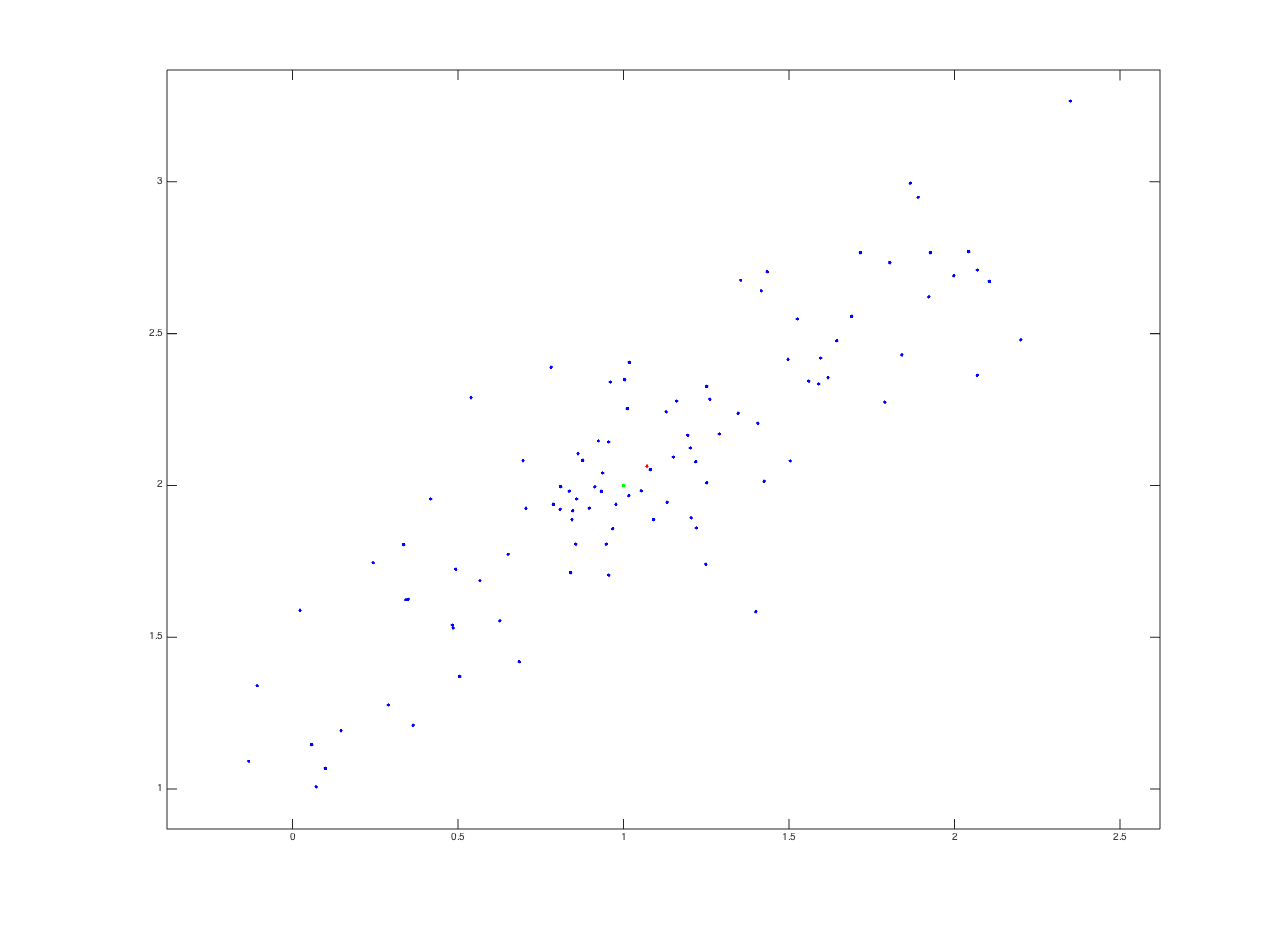
\includegraphics[scale=.3]{img/i23}
\caption{The two means: sample mean (green) and quantitive mean (red) \label{overflow}}
\end{figure}

In Figure 3 we have represented the two means: mu which is the given mean ([1, 2]) and m is the quantitive mean that has been calculated by calculating the average of all the points in the data set. Because we generate the data set randomly, the points are chosen independently from each other. Because of this we have this deviation between the sample mean and the quantitive one. If we would have had a sample that was based on a periodical function, then the mean would have been identical because it would comply to the same rule. Furthermore, the smaller the number of our data set the bigger the deviation gets because we would have larger granularity between the set of values. So if we would have an infinite number of data points we would have "almost" the same mean.\\

\subsection*{I.2.4 Covariance: The geometry of multivariate Gaussian distributions}
The covariance is the property of a function of retaining its form when the variables are linearly transformed. Therefore if we rotate the data set by 30, 60 or 90 degrees we should get the elliptic shape as the standard data set. In our case, the covariance is a matrix of size (2,2).\\
The major axes of the ellipse are defined by the eigenvectors of the covariance matrix, with corresponding eigenvalues.\\

\begin{figure}[h]
\centering
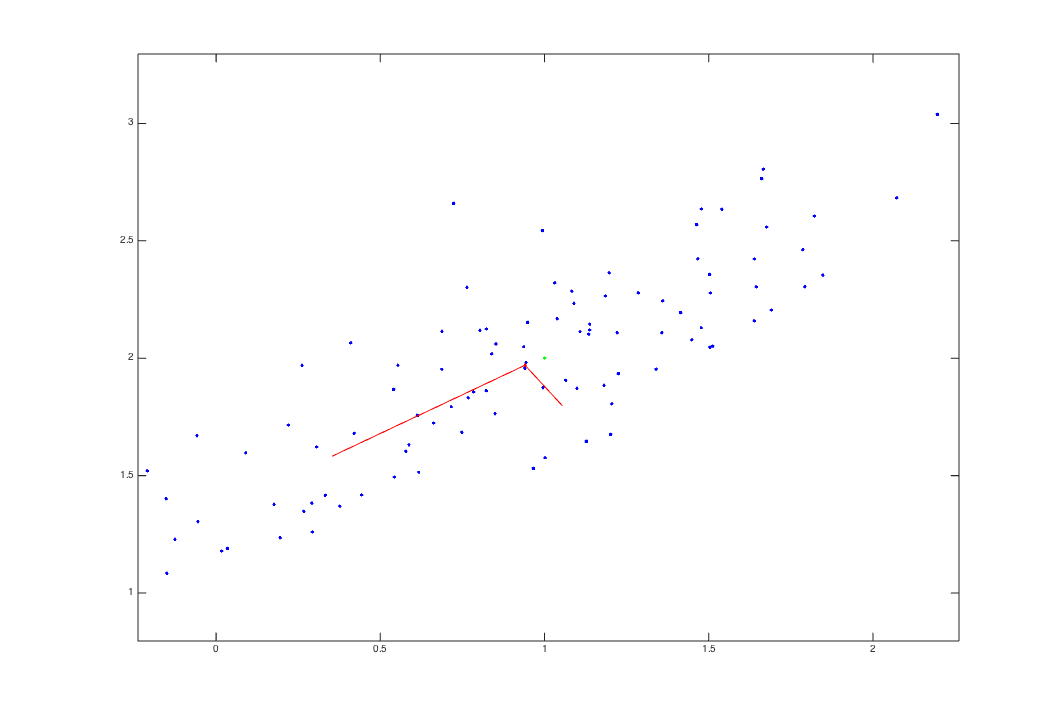
\includegraphics[scale=.3]{img/i24}
\caption{Covariance and eigenvectors \label{overflow}}
\end{figure}

\begin{figure}[h]
\centering
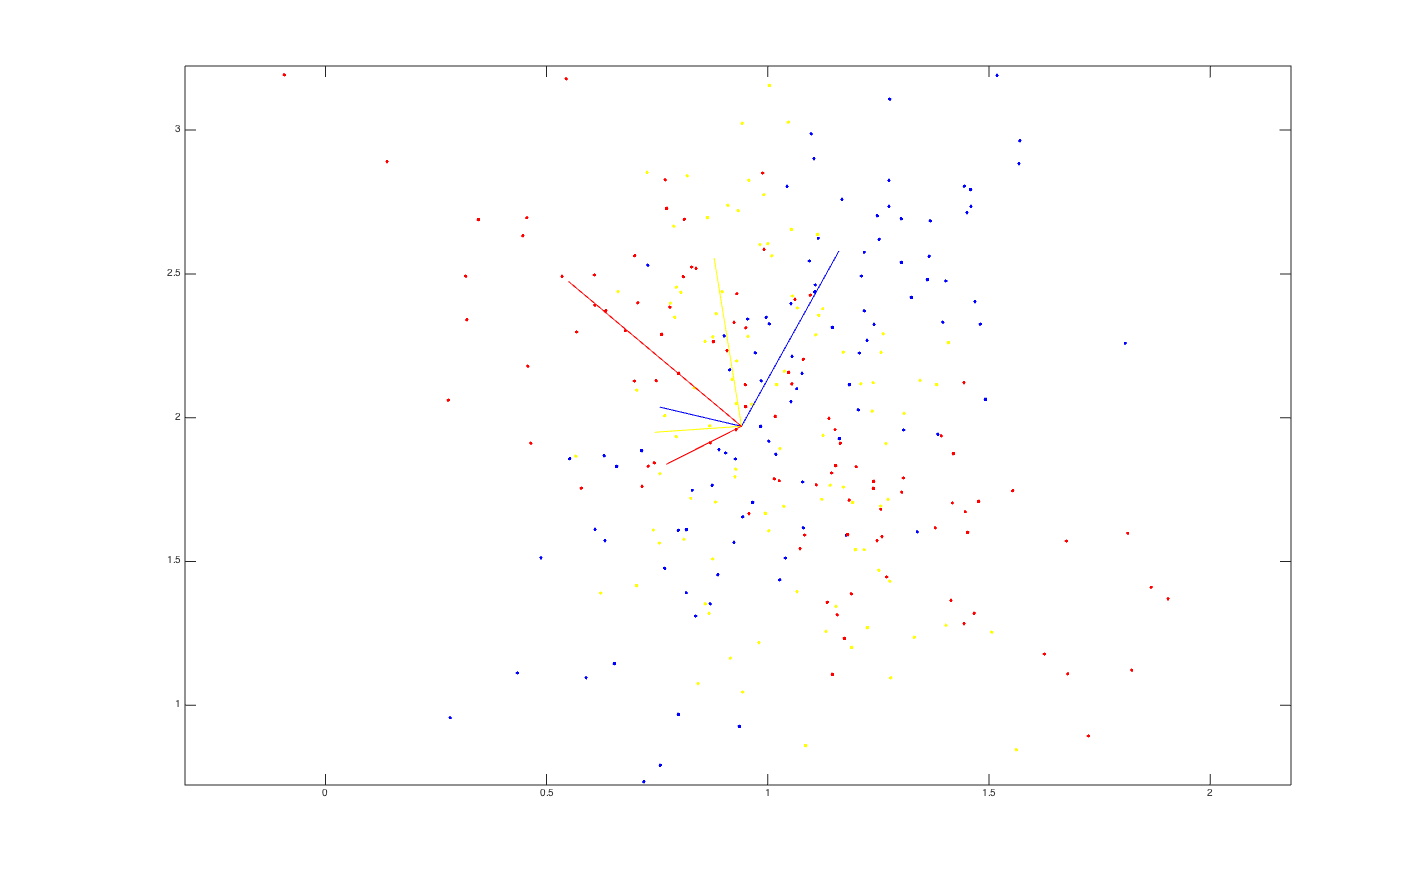
\includegraphics[scale=.3]{img/i24b}
\caption{Combined plot of rotated datasets \label{overflow}}
\end{figure}

\section*{I.3 Classification}
\subsection*{I.3.1 Nearest neighbor}
 
The kNN function is applied for K = {1, 3, 5}. As we can see from Table 1, the best results are for K = 3. The kNN function starts out by calculating the distances for each point in the test data relative ti the train data points. After that we sort the rows by distance and create a counting vector that holds the K number of points that are closest to the current analyzed point. We check then the highest count in the vector and calculate the empirical risk by checking the values from the test data set.\\

\begin{table}[h]
\begin{center}
\begin{tabular}{|
>{\columncolor[HTML]{000000}}c |c|c|c|}
\hline
{\color[HTML]{FFFFFF} \textbf{K}}    & 1      & 3      & 5 \\ \hline
{\color[HTML]{FFFFFF} \textbf{Risk}} & 0.1842 & 0.1842 &  0.3157 \\ \hline
\end{tabular}
\caption{K-NN empirical risk values}
\label{K-NN empirical risk values}
\end{center}
\end{table}

\subsection*{I.3.2 Hyperparameter selection using cross-validation}



\end{document}               % End of document.